\subsection{Client}
Das Frontend besitzt das Design-Muster View-Model-Controler als übergeordnetes Muster. Im Packet \glqq View\grqq{} befinden sich die mit HTML und CSS designten Webseiten. Das Packet \glqq Model\grqq{} dient als Bindeglied zwischen dem \glqq View\grqq{}-Packet und dem \glqq Controller\grqq{}-Paket. Es beinhaltet die Daten die in den Aufbau einer Webseite eingebunden werden und fragt diese an und lässt sie ändern im Packet \glqq Controller\grqq{}. Einen Austausch zwischen dem Frontend und dem Backendserver erfolgt im Packet \glqq Controller\grqq{}. Dies beinhaltet die Daten-, Lösch und Änderungsanfragen.

\begin{figure}[H]
\centerline{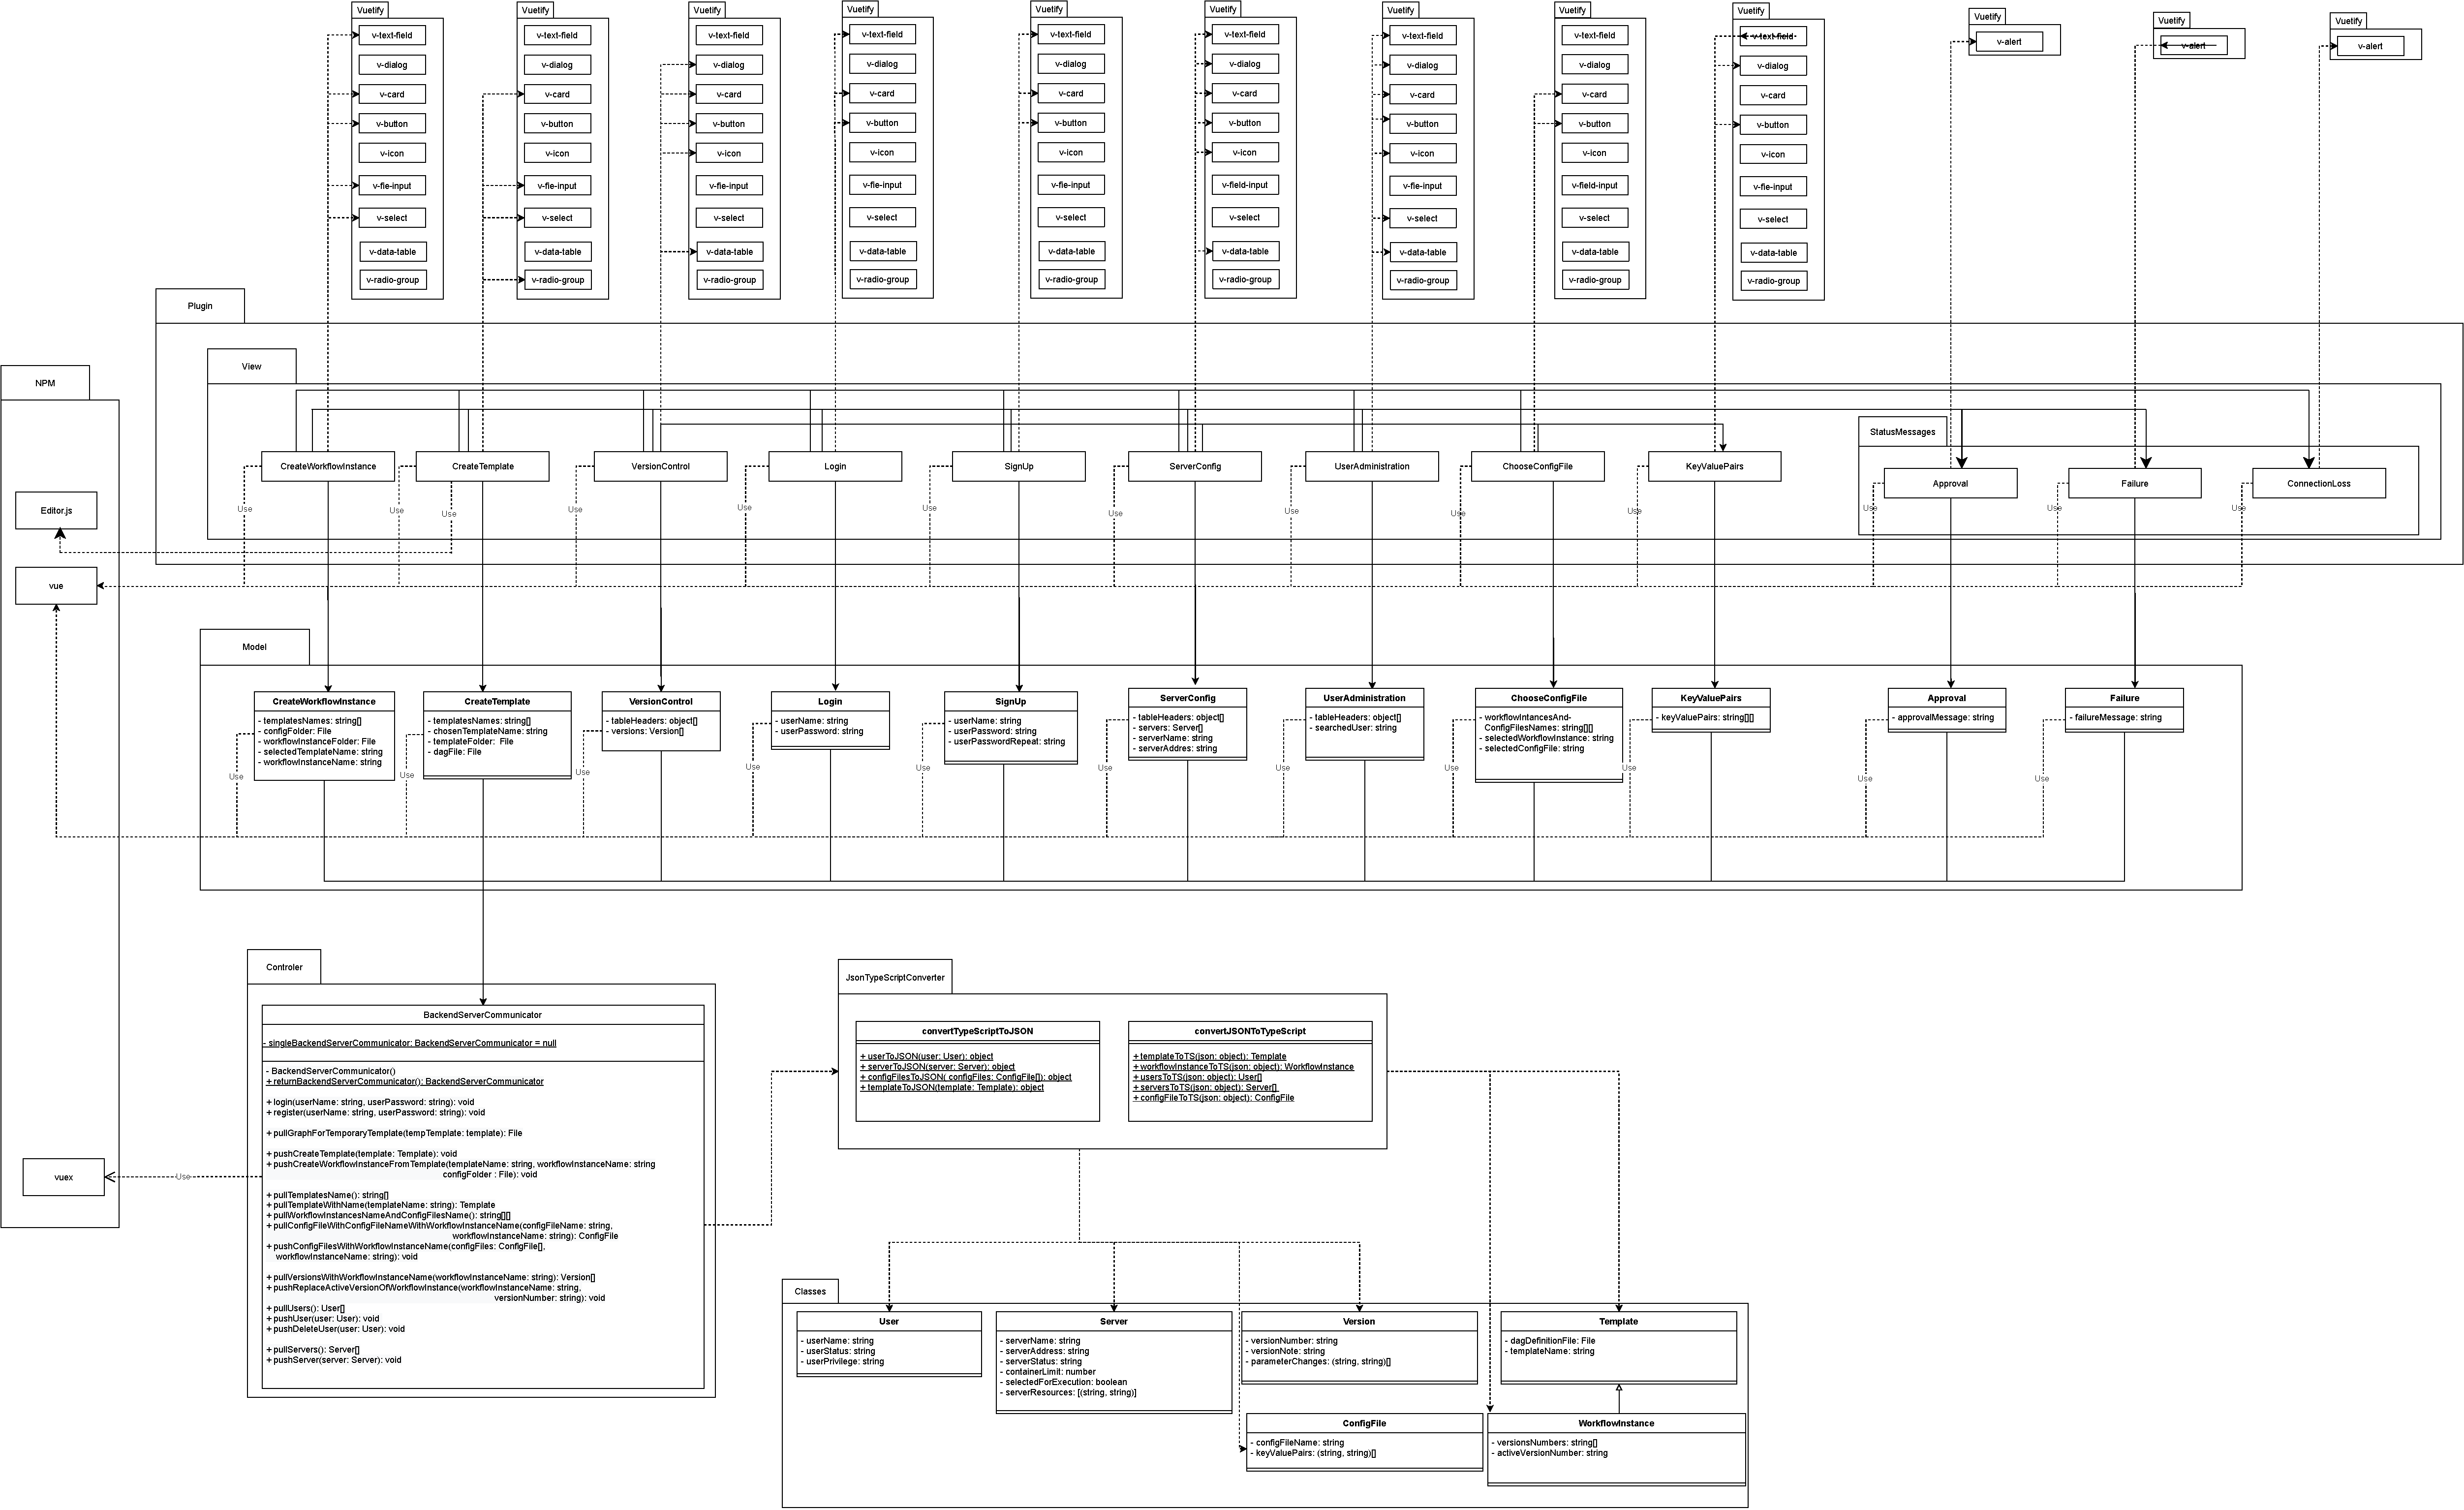
\includegraphics[scale=0.2]{res/FrontendUML.drawio.pdf}}
\caption{Klassendiagramm zum Frontend}
\end{figure}

\newpage